\section{Recommended Simulation Workflow with WESTPA 2.0 Upgrades}

Given the major upgrades in the WESTPA 2.0 software package \citep{russo_westpa_2022}, we recommend the three-stage simulation workflow illustrated in \textbf{Figure 2}. Details of the particular schemes are provided in the tutorials.

% for single column figure don't include the *
\begin{figure}[ht]
\centering
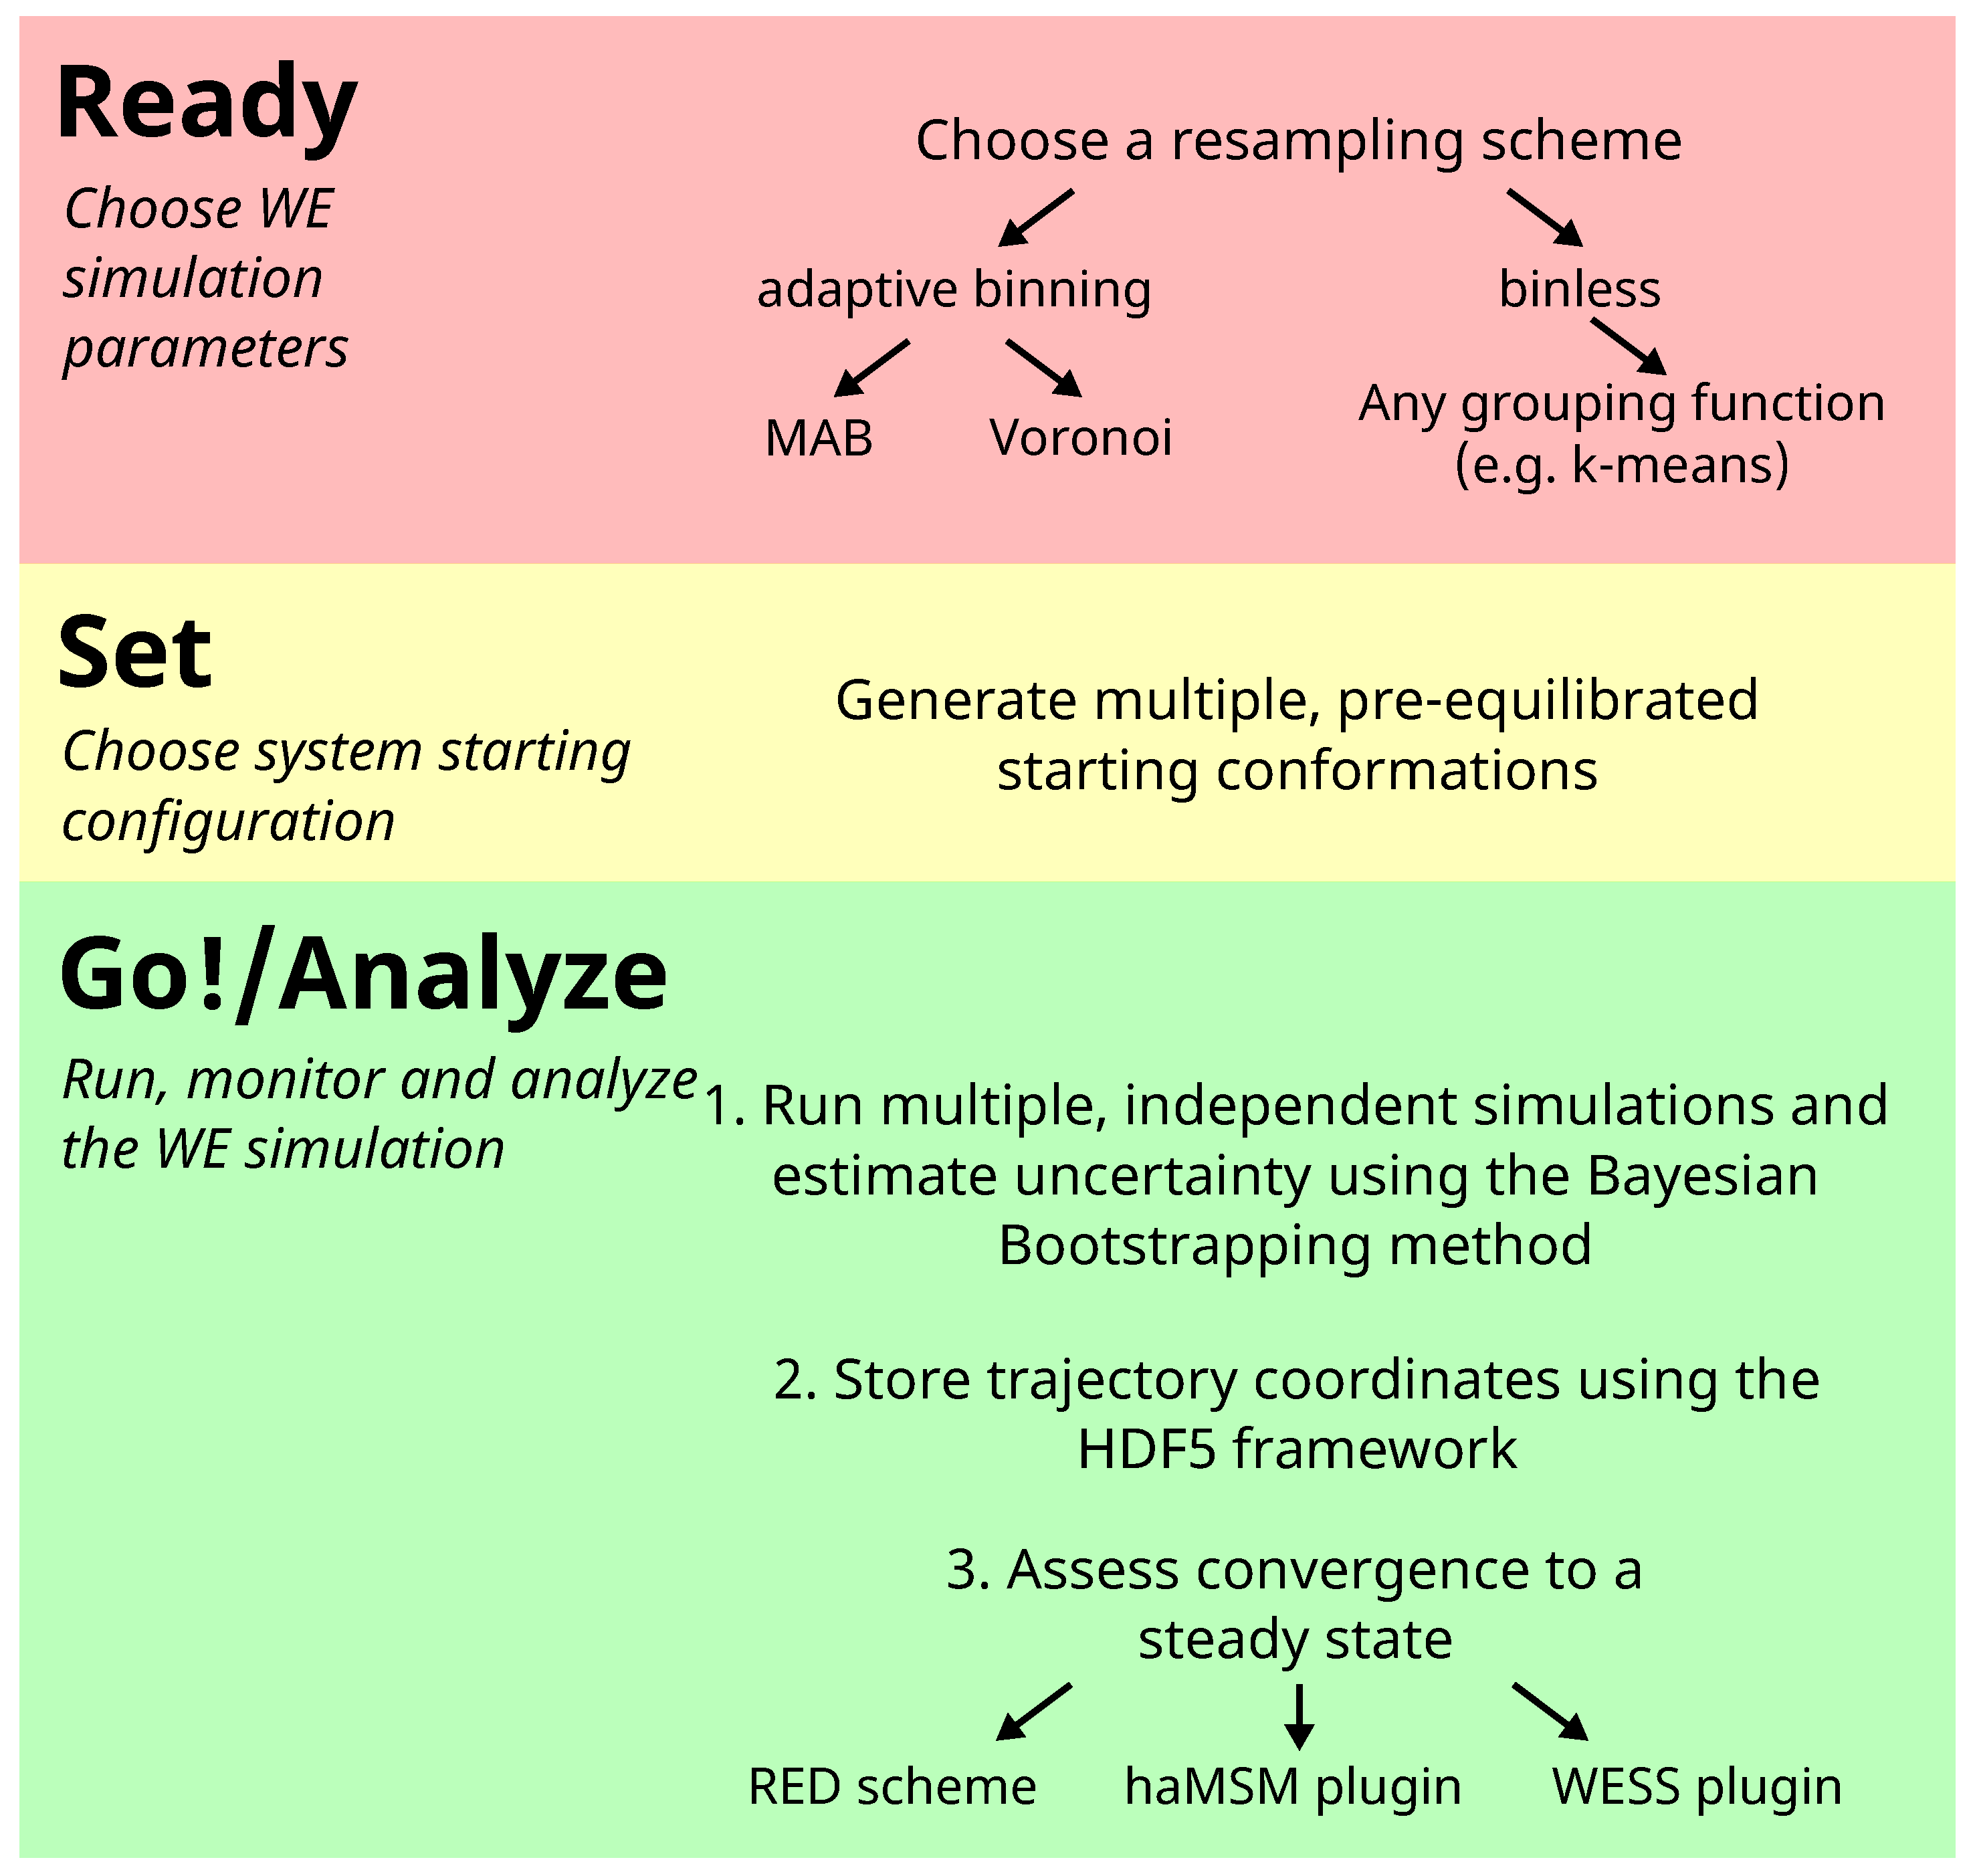
\includegraphics[width=\columnwidth]{figures/Figure2_workflow.pdf}
\caption{Recommended simulation workflow that makes use of major upgrades in the WESTPA 2.0 software.}
\end{figure}

In the first (“Ready”) stage, if one uses a binned resampling scheme, we recommend using one of the two adaptive binning schemes available in WESTPA 2.0: the minimal adaptive binning (MAB) scheme or adaptive Voronoi binning scheme.
These adaptive binning schemes enable quicker explorations of the chosen progress coordinate than manual, fixed binning schemes. 
The MAB scheme is effective at surmounting barriers in a direction of interest \citep{torrillo_minimal_2021} while the adaptive Voronoi binning scheme \citep{zhang_exact_2010} is ideal for enhanced sampling in high-dimensional space (more than three dimensions) when all parts of the progress-coordinate space are potentially important. 
However, if progress-coordinate space includes, for example, undesirable unfolded protein conformations, adaptive Voronoi binning might allocate bins and computing resources to those regions. 
Besides the adaptive binning schemes, one can opt for a “binless” resampling scheme by defining a grouping function as described in \textbf{Advanced Tutorial 3.1} below. 
The choice of $\tau$ (the resampling interval used for your WE simulation) should also be made on a system-by-system basis, with a sufficiently long time interval to capture relevant motions of interest but not so long that no net progress is made toward the target state. 
Examples of tau values used for various systems in previous WE studies are provided in the first suite of WESTPA tutorials \citep{bogetti_suite_2019}. 
Convergence of a WE simulation will ultimately depend on the overall goal of running the simulation, but will most likely involve the time-evolution of an observable of interest leveling off over time (e.g., trajectory flux into a user-defined target state). 
If the convergence criterion is not met, a WE simulation using WESTPA can be resumed by simply running the \verb|./run.sh| script or resubmitting the job if it was originally run with slurm. 
Even if changes were made to the progress coordinate or binning, WESTPA will incorporate those changes and resume the simulation accordingly.

In the second (“Set”) stage, we recommend starting the WE simulation from multiple, pre-equilibrated starting conformations that are representative of the initial stable state (at least one “basis state” for each trajectory walker) to improve the sampling of the initial state and diversity of generated pathways to the target state.
Initial structures for a WE simulation should be chosen on a system-by-system basis, but in general, more starting structures (each with a slightly different initial configuration) should provide you with a more diverse trajectory ensemble. 

In the third (“Go/Analyze”) stage, we recommend applying one of the following three options to further accelerate convergence to a steady state once successful pathways are generated. 
The Rates from Event Durations (RED) analysis scheme \citep{degrave_red_2021} estimates rate constants more efficiently than the original WE scheme \citep{huber_weighted-ensemble_1996} by exploiting information in the transient region of the simulation.
Another option is the haMSM plugin, which employs a fine-grained “microbin” analysis and can be used to not only estimate rate constants following WESTPA simulation (e.g., for the seconds-timescale coronavirus spike opening process \citep{casalino_ai-driven_2021}), but to also restart trajectories with their weights adjusted for a steady state \citep{russo_westpa_2022}. 
Because restarts in the haMSM plugin are initiated from configurations occurring throughout previously run trajectories, the continuity of the generated pathways is broken. 
The third option is the weighted ensemble steady state (WESS) plugin \citep{bhatt_steady-state_2010}, which uses the less fine-grained WE bins to estimate steady state but preserves the continuity of pathways, restarting from only the final points of trajectories. 
While all trajectory files of the chosen dynamics engine are saved by default, we recommend storing the trajectory coordinates using the WESTPA 2.0 HDF5 framework, which greatly facilitates the restarting, storage efficiency, and analysis of WE simulations. 
When possible, users should run multiple WE simulations, which provides a greater number of independent pathways and enables straightforward estimation of error using the Bayesian bootstrap method \citep{mostofian_statistical_2019} (see {\url{https://github.com/ZuckermanLab/BayesianBootstrap}}).  

\textbf{Random Seeds for Simulations.} For WE trajectories to diverge from one another after a splitting event, a stochastic thermostat is required for MD simulations. 
Furthermore, the random number seeds for such thermostats must be sufficiently random (uncorrelated) to avoid undesired bias of the dynamics when trajectories are restarted at short time intervals (e.g., in the case of WE simulations) \citep{cerutti_vulnerability_2008}. 
To avoid such bias, we strongly recommend using WESTPA’s system entropy-seeded random number facility instead of any time-seeded random number generator of the chosen dynamics engine. 
To use this facility, we first set the random seed to \verb|RAND| in the dynamics input file (e.g., \verb|ig=RAND| in the AMBER \verb|md.in| file) and then specify this input file in \verb|runseg.sh|, which will replace the \verb|RAND| string with the WESTPA random number seed. 

\textbf{Extremely Low Trajectory Weights.} While it is possible to set a minimum threshold weight (e.g., 10\textsuperscript{-100}) for trajectories to be considered for splitting, the generation of trajectories with extremely low weights (e.g., <10\textsuperscript{-100}) is a potential warning sign that the division of configurational space is not capturing all relevant free energy barriers. 
If a WE simulation yields such trajectories, we strongly suggest re-evaluating the choice of progress coordinate and/or restricting the binning to a carefully chosen subset of configurational space that would avoid generating such trajectories.
For example of the latter, see \textbf{Advanced Tutorial 3.2}.
